\chapter{Analysis}

In this chapter, we will be doing problem analysis. We will dive deeper into the problem we intend to fix, and why we think it is a problem in the first place. We will discuss various existing approaches at solving the problem, and why these are great efforts. We finish by discussing why believe that the existing approaches fall short of what we aim to achieve.

\section{Problem Definition}

Now is as good a time as any to more concretely outline the problem at hand. Simply put, we aim to portray computer programs at different abstraction levels, without losing the underlying ideas. This can be - and traditionally also has been - done ``manually'' by the program authors. For instance: writing a computer program, testing it, and later rewriting the source code to pseudocode. We believe this is something that comfortabely could, and should, be possible to automate. \hfill \\

There are several use cases where displaying source code with an alternative representation could be useful. Mainly within education, where the goal is to teach students concepts in an agonstic way. However, it could also be used by researchers exchanging ideas, across preferred programming languages. \hfill \\

Already in the 80's Clements et al. predicted that computers would be an integral part of the classroom~\cite{clements1984effects}. Slowly but steady also the art of computer programming has been introduced into school curriculums, at a younger and younger age. While teaching pointers and monads to 10-year-olds, there is a point of introducing them to computer programs integral to the digitalised world we spend our lives in. \hfill \\

If the teacher is to transpile her code to flowcharts, it offers a visual approach to understanding programming concepts. Consequently, the whole classroom can focus more on the underlying logic than on the syntactic quirks of the teacher's preferred programming language. \hfill \\ % Aditionally, the flowcharts should be fairly easy to recreate in an imperative programming language

This is also the case when teaching computer programs at a higher level, for instance in university. Students who already have some experience with programming and reading mathematical notation can still benefit from pseudocode. This also equals the playing field, and avoids putting students who struggle with a specific programming language at a disadvantage. \hfill \\

Lastly, researchers might wish to exchange ideas despite using different programming languages. Just like every animal in the kingdom can be called upon in latin, every idea can be presented with pseudocode. \hfill \\

\forsup{litt tynt?}

In the context of our problem, and the remainder of this thesis, we view flowcharts as a form of pseudocode rather than an isolated concept. As such, we have to make a different distinction between flowcharts and traditional pseudocode which resembles source code. From now, we will refer to traditional pseudocode as \textbf{Text based pseudocode} (TBP) and flowcharts as \textbf{Image based pseudocode} (IBP).



\section{Comparing source code with TBP and IBP}

In this section we aim to show how the same computer program can be presented in three different levels of abstraction, and why TBP and IBP is preferred when strictly focusing on presentation. \\

\forsup{vis AGTI-algoritmen}

\forsup{vis et flowchart hvor man tydelig ser hvordan en algoritme går videre fra mange ifs med return (jeg syns dette kan være kronglete å se i vanlig kode, fordi alt står skrevet sekvensielt!)}

\forsup{vis hvor konsis og kortfattet tbp er i forhold til java eller go. prøv begge, se hvilken av dem som blir styggest hahah}

As such, we can comfortably regard the succinctness of figure 2.1 displaying TBP, to figure 2.2 displaying an implementation of said TBP in a popular programming language \cite{javaIsAPopularProgrammingLanguage}:

\begin{figure}[ht]
    \centering
    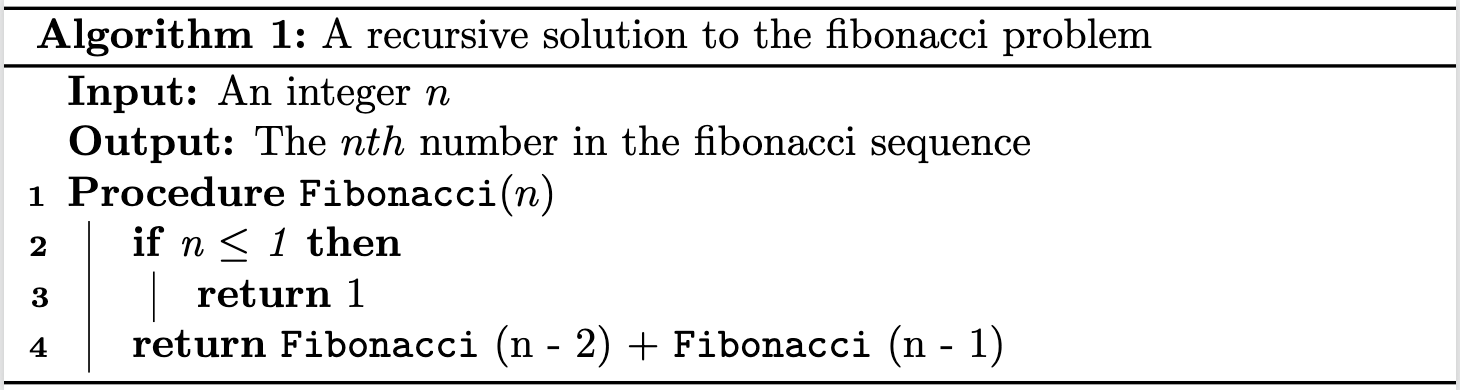
\includegraphics[scale=0.46]{assets/fibonacci_pseudo1.png}
    \caption{Text based pseudocode illustrating an algorithm to retrieve the nth number in a fibonacci sequence.}
    \label{fig:fibseq2}
\end{figure}

\begin{figure}[ht]
    \centering
    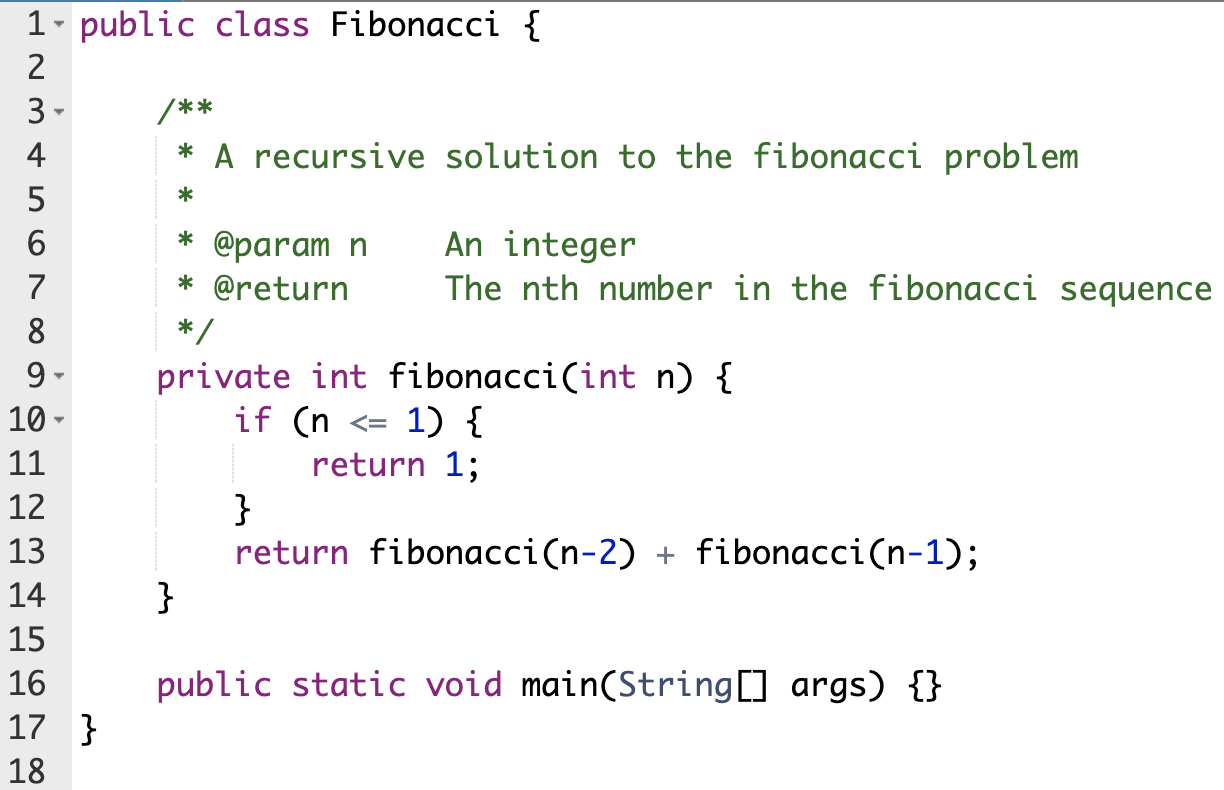
\includegraphics[scale=0.50]{assets/fibonacci_java.png}
    \caption[An algorithm written in the Java programming language, to retrieve the nth number in a fibonacci sequence.]{An algorithm written in the Java programming language, to retrieve the nth number in a fibonacci sequence. It follows the commenting guidlines JavaDoc\footnotemark.}
    \label{fig:fibjava}
\end{figure}
\footnotetext{https://docs.oracle.com/javase/8/docs/technotes/tools/windows/javadoc.html}


The issue of translating code to some sort of pseudo code has been around for a while (source?), often intended to help people less familiar with code, or perhaps those with no familiarity to code whatsoever, to understand what is being done behind the scenes, and better understanding what product is being built etc. (source??). \hfill \\

We, on the other hand, believe that people who \textit{do} have some familiarity with code could also benefit from being exposed to it. For one, it can be a nice tool for debugging a-little-too-fancy code you did not write yourself, by getting a more abstract view of it. It can also aid beginners in seeing the flow of their code, making them understand how they can improve their code. Unfortunately, there does not seem to be any tools freely available on the market with this target audience in mind: people who also code, but would like to see their code from a different perspective. \hfill \\

Another aspect of pseudo code, is that since it is intended to be a presentation-only tool, you cannot actually verify its semantical properties, that is, if it even does what you want it to do. As Donald Knuth famously put it,

\begin{displayquote}
    I have only proven the algorithm correct, not tested it.\cite{DBLP:books/aw/Knuth68}
\end{displayquote}

Therefore, by manually translating executable code into a non-executable form, we are no longer able to test it, and the work of maintaining both quickly turns into a hassle. We believe that everyone benefits from there persisting a stronger relationship between the original code and the presentation-only pseudocode. \hfill \\

Ever since the concept of pseudocode was introduced, there have been attempts at creating tools to automate the process of translating code to pseudocode. The most noteworthy attempt to deliver pseudocode in text format was presented in a 2015 paper, a tool called Pseudogen. When it comes to translating code to flow charts, we decided to look at Code2Flow, which is widely used in practice today, even in PIT, the Norwegian police's IT service. \hfill \\



\section{Related work}

This section will cover selected related work, that has already solved parts of the problem, in their own right. We have separated the section into two further subsections, to analyse efforts related to TBP and IBP individually.

\subsection{Source code to TBP}

Despite TBP being used in so many text books, online courses and published papers, the amount of source-code-to-pseudocode-editors currently available on the internet is anything but overwhelming. Additionally, there is no undisputed choice that is commonly used. There are, however, a couple of candidates who stick out if we look closely enough.

\subsubsection{Naive approach}

The naive approach would be to do this manually. Perhaps the wording is too harsh, but in this context, \texttt{naive} corresponds to \texttt{manual}. By manually writing our own pseudocode, we are void of any restrictions, and can do it just the way we like. \\

The downside is the extra effort in writing both the original algorith, and later also spending time on writing the pseudocode. By doing it manually, we are also forced to maintain both versions.

\subsubsection{Pseudogen}

The Psuedogen transpiler is currently designed to work with a subset of the Python programming language\footnote{https://www.python.org/}. The output target is purely natural language, precisely what you are reading now. As mentioned in Section 2.1.1, the tool is developed using statistical machine translation. This is a technique of translating from one language to another based on statistical models, and is generally used to translate between natural languages \cite{DBLP:conf/kbse/OdaFNHSTN15}. \hfill \\

Despite being a programming language notoriously known for using plain English where many other programming languages use more technical notation ($and$ instead of $\&\&$, $or$ instead of $||$ etc.), Python still bears the mark of being a programming language. People unfamiliar with programming and/or mathematics still might struggle to understand some of the more technical aspects of its syntax. \hfill \\

Figure ?? shows an example taken from the initial 2015 paper where Pseudogen was first presented. It displays Python source code on the left, and pseudocode on the right. The program in question is an algorithm that solves the \textbf{FizzBuzz} problem, a common problem presented in e.g. interview settings. \hfill \\

\begin{figure}[ht]
    \centering
    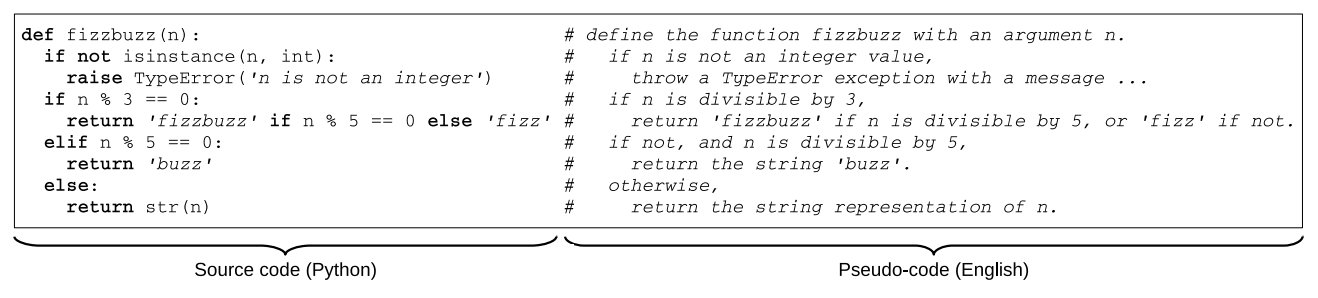
\includegraphics[scale=0.52]{assets/odaetal.png}
    \caption{Example of source code written in Python and corresponding pseudo-code written in English from Oda et. al}
    \label{fig:odaetal}
\end{figure}

What the examples in the 2015 paper, as well as a video on their website\footnote{https://ahclab.naist.jp/pseudogen/} show, is really a line-for-line translation to English. This could be desired in cases where the business people on the team are particularly curious about what the product is really doing under the hood (and the boss cannot afford Cobol developers). \\

However, since Pseudogen will translate each line in a slave-like manner, we also translate all error handling of a ``real'' program. Listing ?? shows some error handling in Python, and Listing ?? shows the result from transpiling it with Pseudogen. \\

\begin{lstlisting}[caption={Error handling in Python}, captionpos=b, frame=trbl]
    except ValueError as e:
        print(e)
\end{lstlisting}

\begin{lstlisting}[caption={The result of transpiling the code in Listing ?? with Pseudogen}, captionpos=b, frame=trbl]
    # If ValueError, renamed to e, exception is caught.
        # Call the function print with an argument e.
\end{lstlisting}

The results tend to be overwhelmingly verbose, which also defeats much of the point with Python. Programs in the language tend to be elegant and succinct, and already closely resemble natural language. \hfill \\

Another example is visible in Listing ?? and Listing ??, where list comprehension has been translated very literally. It is plausible to assume people with backgrounds in e.g. mathematics might favour the Python version to the transpiled one. \hfill \\

\begin{lstlisting}[caption={A list comprehension of applying f(n) to integers in the range -10 to 10, and placing the results in a list}, captionpos=b, frame=trbl]
    a = [f(n) for n in range(-10, 10)]
\end{lstlisting}

\begin{lstlisting}[caption={The result of transpiling the code in Listing ?? with Pseudogen}, captionpos=b, frame=trbl]
    # Call the function f with an argument n for every
      n in range of integers from range 10 negative
      integer 10, substitute the result for a
\end{lstlisting}

It is clear that the target audience for Pseudogen's output formats must be people with little to no experience with reading/writing code. It seems like an excellent tool for translating Python to English, and shows that something like this is indeed possible. However, Psnodig's intended target audience is broader, and thus we believe Pseudogen alone is not enough to satisfy our needs.

\subsubsection{PseudoEditor}

\forsup{Har ikke fått denne til å funke enda! Gir ikke mening}


\subsection{Source code to IBP}

Even though there is research arguing for the good effects of flowcharts in computer science, there have been few documented efforts towards developing a tool that can effectively translate source code to flowcharts. However, there does exist some software that lets us write flowcharts through a DSL, and we will look at two of them.

\subsubsection{Naive approach}

Yet again, calling it a naive approach might not be entirely accurate, but manually translating our code to flowcharts does introduce some intricacies. For one, like with TBP, we have to maintain both versions, and if we change too much of our main idea, then the time spent on making the IBP version is - to a certain extent - wasted. \\

Another flaw is that we have to spend time thinking about how the flowchart should look like, which parts could and should be abstracted, how they should be presented instead (or if they should be removed altogether) etc. Which colours should the frames have? How should the arrows look? Which font should be used? By using an automated tool, we do not have to worry about details unrelated to the actual program. \\

The perk of doing it this way, however, is that we can do it entirely our way. We can choose which tools we want to use, and if we are already proficient, then this seems like a natural choice. If we also like spending time on details like colours, fonts, shapes etc., then at least the naive approach does not limit our creativity in any way. \\

\forsup{Jeg føler egentlig at det er naturlig å starte med det positive, og avslutte med det negative?}

\subsubsection{Code2Flow}

Code2Flow is a tool that lets us create flowcharts with natural language, decorated with a C-inspired syntax. Their website states that we might get away with pasting C programs, but that this is purely incidental, indicating that they have indeed developed a DSL with their own syntax. \\

Flowcharts created with Code2Flow have a few, consistent colours to differentiate parts of their corresponding programs. Start- and end expressions are displayed as red ovals, while all other expressions are displayed as blue rectangles. Conditionals, loops and match statements are displayed with red rhombuses, and comments are displayed with orange rectangles. \\

\begin{figure}[ht]
    \centering
    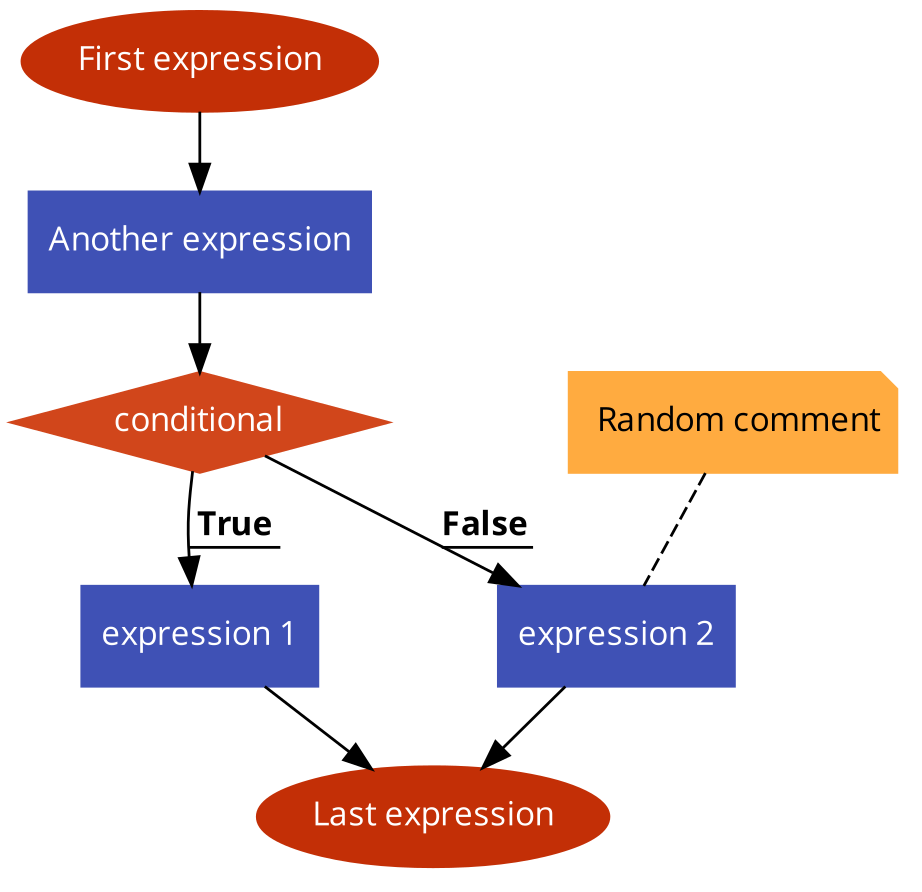
\includegraphics[scale=0.2]{assets/code2flow_example.png}
    \caption{The resulting flowchart from transpiling the Code2Flow code in Listing ??}
    \label{fig:code2flow}
\end{figure}

Listing ?? shows a program written with Code2Flow, and Figure ?? shows the corresponding flowchart. As we can see, syntactically correct expressions are just any combination of UTF-8 characters. Thus, we have no way to test a Code2Flow program. In fact, Code2Flow will \textit{never} let us know about syntactic errors, and always try to construct whatever flowchart it can. \\

\begin{lstlisting}[caption={A Code2Flow program}, captionpos=b, frame=trbl]
    First expression;
    Another expression;
    if (conditional) {
      expression 1;
    } else {
      expression 2; // Random comment
    }
    Last expression;
\end{lstlisting}

If our C program inadvertently creates a ``correct'' flowchart, we can use a C compiler to test said program on the side. However, we must now maintain both versions, and changes to the C program are not guaranteed to successfully transpile to a flowchart. \\

\subsubsection{Mermaid.js}

Mermaid.js is a DSL for rendering diagrams (including flowcharts) from a Markdown-inspired syntax. Even though they make many different diagrams, we will focus on the flowcharts. \\

Like Code2Flow, they also render flowcharts in real time. However, Mermaid.js will warn us about syntax errors, and only re-render syntactically correct programs. \\

To write a Mermaid.js flowchart, the code has to start with \texttt{flowchart TD}. Nodes can come in many different shapes, and are denoted by the types of brackets they use. For instance, \texttt{Node[ ]} displays a rectangle, \texttt{Node(( ))} displays a circle, and \texttt{Node\{ \}} displays a rhombus. Edges also come in many shapes. \texttt{-->} displays an arrow, \texttt{---} displays a simple link, and \texttt{-.->} displays a dotted arrow. We can also have add text, by doing e.g. \texttt{Node[text]} or \texttt{-- text -->}. The full documentation can be found at~\url{https://mermaid.js.org/syntax/flowchart.html}. \\

\begin{lstlisting}[caption={A mermaid.js program}, captionpos=b, frame=trbl]
    flowchart TD
        A([First expression])
            --> B[Another expression]
        B --> C{contidional}
        C -- True --> D[Expression 1]
        C -- False --> E[Expression 2]
        D --> F([Last expression])
        E --> F
\end{lstlisting}

Just like with Code2Flow, the text inside these nodes can be anything. Listing ?? shows a program written with Mermaid.js, and Figure ?? shows the corresponding flowchart. Contrary to Code2Flow, comments are ignored by the parser, and solely exist to ait the programmer. \\

\begin{figure}[ht]
    \centering
    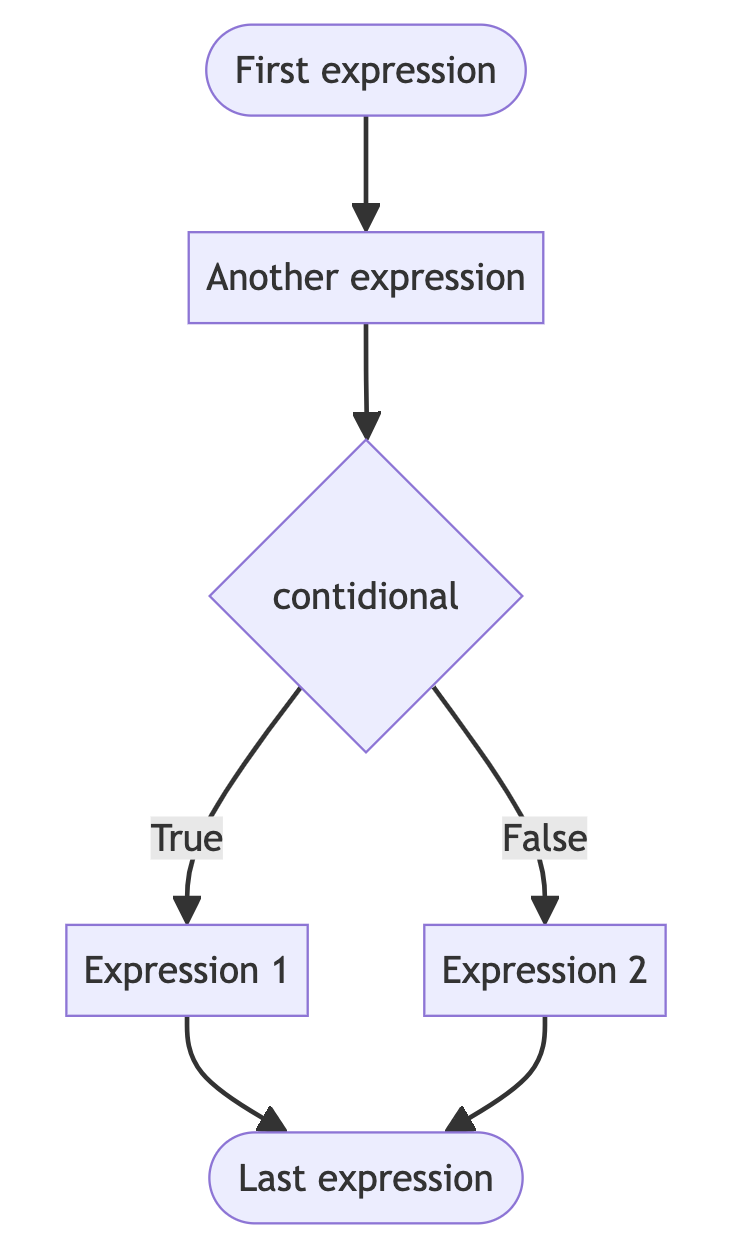
\includegraphics[scale=.5]{assets/mermaidjs.png}
    \caption{The resulting flowchart from transpiling the Mermaid.js code in Listing ??}
    \label{fig:code2flow}
\end{figure}

The biggest drawback of Mermaid.js, is that the syntax is very different from any programming language. This means pasting our source code will not yield any result, and we have to carefully translate our code every time. This means that it is fully our responsability to maintain the abstraction level we want. Like Code2Flow, Mermaid.js has no way of letting us test the code either.